\documentclass[a4paper]{article}
\usepackage[UTF8]{ctex}
\usepackage[top=2mm,bottom=2mm,left=2mm,right=2mm]{geometry}
\usepackage{amsmath,amssymb,bm,multicol,graphicx,xcolor,tikz,array,tabularx}
\usetikzlibrary{arrows.meta}
\pagestyle{empty}
\setlength{\parindent}{0pt}
\setlength{\parskip}{0pt}
\setlength{\columnsep}{1.25mm}
\setlength{\columnseprule}{0.12pt}
\setlength{\tabcolsep}{1pt}
\setlength{\fboxsep}{0.35pt}
\renewcommand{\baselinestretch}{0.66}
\definecolor{h}{RGB}{0,64,150}
\definecolor{s}{RGB}{0,92,175}
\definecolor{r}{RGB}{180,40,30}
\definecolor{g}{RGB}{0,120,70}
\definecolor{bg}{RGB}{238,244,252}
\definecolor{warnbg}{RGB}{255,244,236}
\definecolor{grid}{RGB}{185,198,218}
\newsavebox{\fitbox}
\newcommand{\fitmath}[2][\dimexpr\linewidth-3pt\relax]{\sbox{\fitbox}{$\displaystyle #2$}\ifdim\wd\fitbox>#1\resizebox{#1}{!}{$\displaystyle #2$}\else\usebox{\fitbox}\fi}
\newcommand{\F}[1]{\colorbox{bg}{\fitmath{#1}}}
\newcommand{\mother}[1]{\vspace{0.25pt}\noindent{\fontsize{6.1}{6.25}\selectfont\bfseries\color{white}\colorbox{h}{\strut\ #1\ }}\par\vspace{0.15pt}}
\newcommand{\child}[5]{\vspace{0.18pt}\noindent\fcolorbox{grid}{white}{\begin{minipage}{0.982\linewidth}\fontsize{4.23}{4.42}\selectfont\textbf{\color{s}#1}\par\textbf{触发}：#2\par\textbf{第一行}：#3\par\textbf{顺序}：#4\par\textbf{收口}：#5\end{minipage}}\par}
\newcommand{\tinybox}[2]{\vspace{0.16pt}\noindent\fcolorbox{grid}{white}{\begin{minipage}{0.982\linewidth}\fontsize{4.18}{4.36}\selectfont\textbf{\color{s}#1}\par #2\end{minipage}}\par}
\newcommand{\warnbox}[1]{\vspace{0.12pt}\noindent\colorbox{warnbg}{\begin{minipage}{0.982\linewidth}\fontsize{4.12}{4.30}\selectfont\textbf{\color{r}收口检查}：#1\end{minipage}}\par}
\newcommand{\pipepic}{\begin{center}\begin{tikzpicture}[>=Latex,scale=.34,every node/.style={font=\tiny}]
\draw[blue,->] (-.2,0)--(.7,0);\draw[thick] (0,-.25)--(1.2,-.25)--(1.2,.25)--(2.1,.25);\draw[thick] (0,.25)--(1.2,.25);\draw[thick] (2.1,.25)--(2.1,-.25)--(1.2,-.25);\draw[thick] (2.1,0)--(3.1,0);\node at (1.15,.55){泵/阀/弯头};\node at (2.7,.35){出口};\end{tikzpicture}\end{center}\vspace{-3pt}}
\newcommand{\pvzpic}{\begin{center}\begin{tikzpicture}[>=Latex,scale=.31,every node/.style={font=\tiny}]
\draw[fill=gray!15,draw=black] (0,0) rectangle (.9,1.45);\draw[fill=gray!15,draw=black] (4.4,0) rectangle (5.25,.85);
\draw[dashed] (.1,1.2)--(5.1,1.2);\draw[dashed] (.1,.45)--(5.1,.45);
\draw[thick] (.9,.36)--(2.15,.36)--(2.15,.54)--(.9,.54);
\draw[thick] (2.15,.28)--(4.4,.28)--(4.4,.62)--(2.15,.62);
\draw[blue,->] (1.15,.45)--(3.85,.45);
\draw[<->] (.45,.45)--(.45,1.2);\node[left] at (.45,.83){\(H\)};
\draw[<->] (4.85,.85)--(4.85,1.2);\node[right] at (4.85,1.03){\(h\)};
\node at (1.25,.25){A细};\node at (3.25,.2){B粗};\node at (2.15,.82){突扩};\node at (.45,1.38){C};\node at (4.85,1.02){D};
\end{tikzpicture}\end{center}\vspace{-3pt}}
\newcommand{\gatepic}{\begin{center}\begin{tikzpicture}[>=Latex,scale=.34,every node/.style={font=\tiny}]
\draw[fill=blue!8] (0,0) rectangle (1.3,1.5);\draw[thick] (1.3,0)--(1.8,.35)--(1.8,1.15)--(1.3,1.5);\draw[->] (1.75,.75)--(2.5,.75);\node at (.65,1.7){水深};\node at (2.3,1.25){闸门};\end{tikzpicture}\end{center}\vspace{-3pt}}
\newcommand{\cvpic}{\begin{center}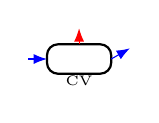
\begin{tikzpicture}[>=Latex,scale=.34,every node/.style={font=\tiny}]
\draw[thick,rounded corners] (0,0) rectangle (2.4,1.1);\draw[blue,->] (-.7,.55)--(0,.55);\draw[blue,->] (2.4,.55)--(3.1,.95);\draw[red,->] (1.2,1.1)--(1.2,1.7);\node at (1.2,-.25){CV};\end{tikzpicture}\end{center}\vspace{-3pt}}
\newcommand{\lavalpic}{\begin{center}\begin{tikzpicture}[>=Latex,scale=.34,every node/.style={font=\tiny}]
\draw[thick] (0,.55)..controls(1,.4)and(1.4,.18)..(2,.18)..controls(2.6,.18)and(3,.4)..(4,.55);
\draw[thick] (0,-.55)..controls(1,-.4)and(1.4,-.18)..(2,-.18)..controls(2.6,-.18)and(3,-.4)..(4,-.55);
\draw[blue,->] (-.4,0)--(.6,0);\draw[blue,->] (3.4,0)--(4.4,0);\draw[red] (2,-.45)--(2,.45);\node at (2,-.75){喉 \(A^*\)};\node at (.4,.85){\(p_0,T_0\)};\node at (3.6,.85){\(p_e,p_b\)};\end{tikzpicture}\end{center}\vspace{-3pt}}
\newcommand{\shockpic}{\begin{center}\begin{tikzpicture}[>=Latex,scale=.34,every node/.style={font=\tiny}]
\draw[blue,->] (0,0)--(1.2,0);\draw[thick] (1.2,-.35)--(3,.2);\draw[red] (1.6,-.4)--(2.1,.45);\node at (.6,.35){\(M_1\)};\node at (2.2,.65){\(\beta\)};\node at (2.8,-.15){楔角};\end{tikzpicture}\end{center}\vspace{-3pt}}
\newcommand{\platepic}{\begin{center}\begin{tikzpicture}[>=Latex,scale=.34,every node/.style={font=\tiny}]
\draw[blue,->] (0,.8)--(1,.8);\draw[thick] (0,0)--(3,0);\draw[red] (0,0)..controls(.7,.15)and(1.7,.45)..(3,.9);\node at (1.5,-.25){平板边界层};\node at (2.5,.65){\(\delta(x)\)};\end{tikzpicture}\end{center}\vspace{-3pt}}
\begin{document}
\fontsize{4.28}{4.48}\selectfont
\begin{multicols}{3}

\mother{母题1 管路机械能：水池--管路--泵--水轮机--汽蚀}
\pipepic
\pvzpic
\child{子题1.0 两油箱/水池--变径管PVZ母型}
{两容器液面有高差 \(h\)，中间一段细管一段粗管，有入口、出口、突扩、阀/弯头，问流量或 A/B 点压强。}
{第一行固定写：\(\displaystyle {p_1\over\rho g}+\alpha_1{V_1^2\over2g}+z_1={p_2\over\rho g}+\alpha_2{V_2^2\over2g}+z_2+h_L\)。简记就是左边 PVZ = 右边 PVZ + 损失。}
{大容器液面 \(p=0\) 表压、\(V\approx0\)。细管 \(V_s=Q/A_s\)，粗管 \(V_b=Q/A_b\)。损失按所在管段取速度：入口 \(0.5V_s^2/2g\)，出口 \(1.0V_b^2/2g\)，突扩 \((V_s-V_b)^2/2g\)，沿程 \(\lambda L V^2/(d2g)\)。}
{管轴线作基准则管内点 \(z=0\)。所有 \(P\) 项写 \(p/\rho g\)，最后要把水头换回 Pa：\(p=\rho g(p/\rho g)\)。}
\child{子题1.0a PVZ母型第一步：两液面求 \(Q\)}
{题问输油流量/输水流量，且左右两端都是大容器液面。}
{取左液面 C 到右液面 D：\(z_C-z_D=h=h_L\)。}
{短管忽略沿程时：\(h=0.5V_s^2/(2g)+(V_s-V_b)^2/(2g)+1.0V_b^2/(2g)\)，且 \(V_b=Q/A_b,\ V_s=Q/A_s\)。长管时再加 \(\lambda_1L_1V_s^2/(d_1 2g)+\lambda_2L_2V_b^2/(d_2 2g)\)。}
{这一步只负责定 \(Q\)。不要把 A/B 点压力提前塞进去；液面方程没有 \(p_A,p_B\)。}
\child{子题1.0b PVZ母型第二步：求细管 A 点压强}
{题问 A 点在细管内，A 在入口之后、突扩之前。}
{从左液面 C 列到 A：\(H={p_A\over\rho g}+{V_s^2\over2g}+h_{e}+h_{f,CA}\)。}
{若短管忽略沿程且 A 在入口后：\(H={p_A\over\rho g}+(1+0.5){V_s^2\over2g}\)，所以 \(p_A/\rho g=H-1.5V_s^2/(2g)\)。若 A 前有长度，另加 \(\lambda L_{CA}V_s^2/(d_s2g)\)。}
{\(p_A\) 可为负表压；只要绝压仍高于汽化压就不一定错误。题目要“压强”时说明表压还是绝压。}
\child{子题1.0c PVZ母型第二步：求粗管 B 点压强}
{题问 B 点在粗管内，B 在突扩之后、出口之前。}
{最省力通常从 B 列到右液面 D：\({p_B\over\rho g}+{V_b^2\over2g}+z_B=z_D+h_{L,BD}\)。}
{若 B 到右液面之间忽略沿程，只剩出口损失 \(1.0V_b^2/(2g)\)，且右液面比管轴高 \(H-h\)，则 \({p_B\over\rho g}=H-h\)。若 B 到出口有长度，则 \({p_B\over\rho g}=H-h+\lambda L_{BD}V_b^2/(d_b2g)\)（按选点方向检查符号）。}
{B 是粗管，用 \(V_b\)，不是 \(V_s\)。局部损失永远取该局部件所属前后规定的速度，突扩单独用 \((V_s-V_b)^2/2g\)。}
\child{子题1.0d PVZ母型长管：给 \(Q\) 反求液面差 \(h\)}
{题给目标流量 \(Q\)、两段长度、粗糙度，问上下游液面差或所需水头。}
{直接算 \(V_s,V_b,Re_s,Re_b\)，再求 \(\lambda_s,\lambda_b\)。}
{层流：\(\lambda=64/Re\)。湍流：按题给 Colebrook/对数式 \(\displaystyle {1\over\sqrt{\lambda}}=-2\log\left({\varepsilon/d\over3.7}+{2.51\over Re\sqrt{\lambda}}\right)\) 迭代。最后 \(h=\sum h_f+\sum h_\zeta\)。}
{粗糙度只进沿程损失；入口、出口、突扩这些局部损失不靠粗糙度。}
\child{子题1.1 水池到出口求流量 \(Q\)}
{大水池、长管、出口大气、给水位差/管长/直径/局部件，问 \(Q\)。}
{取1为上游自由面，2为出口截面；写修正Bernoulli，表压 \(p_1=p_2=0\)，大水面 \(V_1\approx0\)。}
{\(V=Q/A\to Re=Vd/\nu\to\lambda\to H=V^2/2g+\lambda(L/d)V^2/2g+\sum\zeta V^2/2g\to Q=AV\)。若\(\lambda\)未知，用试算--查Moody--迭代。}
{出口速度头不能漏；局部损失永远非负；\(m^3/h\)先除3600；直径mm先转m。}
\child{子题1.2 已知 \(Q\) 求某点压强或压力表读数}
{题给流量、压力表、测压点、某截面压强，问 \(p\) 或表压。}
{沿已知压强截面到未知截面列机械能方程；全部用表压时，大气相通点取0。}
{\(Q\to V_i=Q/A_i\to Re_i\to \lambda_i\to h_L=\sum\lambda_iL_iV_i^2/(d_i2g)+\sum\zeta_iV_i^2/(2g)\to p_x/\rho g\)。}
{压力表给表压；若题涉及汽化压必须转绝压；不同管径不能共用一个 \(V\)。}
\child{子题1.3 泵扬程、泵功率、效率}
{水泵、扬程、轴功率、效率、输水、泵前后压力表。}
{在能量方程中给流体加 \(+H_p\)：\(z_1+p_1/\rho g+V_1^2/2g+H_p=z_2+p_2/\rho g+V_2^2/2g+h_L\)。}
{先由方程求 \(H_p\)；水功率 \(P_w=\rho gQH_p\)；轴输入 \(P_s=P_w/\eta\)。若给轴功率，反算 \(H_p=\eta P_s/(\rho gQ)\)。}
{别把效率乘反；泵让总水头上升，算出负扬程要查截面方向。}
\child{子题1.4 水轮机输出功率}
{水轮机、发电、输出功率、上游下游水位/压力。}
{水流失去机械能，写 \(z_1+p_1/\rho g+V_1^2/2g=z_2+p_2/\rho g+V_2^2/2g+h_L+H_T\)。}
{\(H_T=\)上游总水头--下游总水头--损失；轴输出 \(P_{\rm out}=\eta\rho gQH_T\)。}
{题问“水流给转轮的功率”通常不乘效率；题问轴功率才乘效率。}
\child{子题1.5 泵吸水高度/汽蚀}
{泵高于水面、汽化压、入口压至少高于汽化压、安全余量、最大安装高度。}
{从吸水池自由面1列到泵入口2：\(p_2=p_a-\rho g(z_2-z_1)-\rho V^2/2-\rho gh_L\)。}
{\(Q\to V\to Re,\lambda,h_L\)，令 \(p_2\ge p_v+\Delta p_{\rm safe}\)，解最大 \(h=z_2-z_1\)。}
{全程用绝压；吸入段入口阀、弯头、沿程都算；高度越大越危险。}
\child{子题1.6 粗糙度、Moody、沿程损失}
{镀锌钢管、铸铁、粗糙度 \(\varepsilon\)、水温、运动粘度、压降反推。}
{先判 \(Re\)：层流 \(Re<2300\) 直接 \(\lambda=64/Re\)；湍流用 \(Re,\varepsilon/d\) 查Moody。}
{\(h_f=\lambda(L/d)V^2/(2g)\)，压降 \(\Delta p=\rho gh_f\)。若已知压降反推粗糙度：方程先解 \(\lambda\)，再由 \(Re,\lambda\) 查 \(\varepsilon/d\)。}
{Moody中的 \(\lambda\)通常是Darcy系数；不要把局部损失系数 \(\zeta\) 当 \(\lambda\)。}
\child{子题1.7 串联、并联、多管径}
{不同直径、多段管、并联支路、分流、汇流。}
{先画节点和截面；串联同 \(Q\)，并联同两端水头差。}
{串联：每段 \(V_i=Q/A_i,Re_i,\lambda_i\)，损失相加。并联：设 \(Q_a,Q_b\)，列 \(Q=Q_a+Q_b\)，且 \(h_{La}=h_{Lb}\)。}
{并联损失不是相加；局部件用所在管段速度头。}
\child{子题1.8 文丘里、孔板、喷嘴测流}
{差压计、孔板、文丘里管、喷嘴、流量系数 \(C_d\)。}
{取上游1和喉/孔口2，写Bernoulli和连续方程。}
{理想文丘里 \(Q=A_2\sqrt{2\Delta p/[\rho(1-(A_2/A_1)^2)]}\)；实际乘 \(C_d\)。孔口常用 \(Q=C_dA\sqrt{2gH}\)。}
{差压计先换成 \(\Delta p\)；孔板损失大，文丘里损失小。}
\child{子题1.9 图里有压力表：截面压强不能乱省}
{管路图上某截面装压力表，题问压力表读数、另一点压力、或用压力表求机器水头。}
{把压力表所在截面当成普通截面：\(\displaystyle H_i={p_i\over\rho g}+{V_i^2\over2g}+z_i\)。}
{压力表读数通常是表压，可直接作为 \(p_i\) 进入水力能量方程；但若后面判断汽蚀、蒸汽压、气体状态方程，必须转绝压 \(p_{\rm abs}=p_g+p_a\)。若该截面管径变化，先用 \(V_i=Q/A_i\)。}
{压力表截面有速度头，不能把它当大水池液面。表压可以为负，绝压不能为负。}
\child{子题1.10 图里有阀门、弯头、入口、出口：局部损失归位}
{题图标入口阀、弯头、闸阀、出口、突然扩大/缩小，或者直接给 \(\zeta,K\)。}
{第一行写 \(h_L=h_f+\sum h_\zeta\)，再逐个局部件列出。}
{入口 \(h_e=K_eV^2/2g\)，出口 \(h_o=K_oV^2/2g\)，阀/弯头 \(h_\zeta=\zeta V^2/2g\)。突扩不用 \(\zeta V^2/2g\) 时写 \(h=(V_1-V_2)^2/2g\)。不同管径时，局部件在哪段就用哪段速度；突扩/突缩用前后速度。}
{长管有时可忽略局部损失，短管局部损失常不能忽略；题给 \(K,\zeta\) 就必须用。}
\child{子题1.11 图里有粗糙度：只服务于沿程损失}
{题给镀锌钢管、铸铁管、粗糙度 \(\varepsilon\) 或 \(h\)，要求压降、流量、液面差。}
{先算相对粗糙度 \(\varepsilon/d\)，再算 \(Re=Vd/\nu\)。}
{层流：\(\lambda=64/Re\)，粗糙度不进入。湍流：用 \(Re,\varepsilon/d\) 查 Moody 或用 Colebrook。完全粗糙区 \(\lambda\) 近似只随 \(\varepsilon/d\) 变。反求粗糙度时：先由能量方程求 \(\lambda\)，再用 \(Re,\lambda\) 反读 \(\varepsilon/d\)。}
{粗糙度不是局部损失系数；\(\lambda,\zeta,C_D,C_f\) 四个符号不能混用。}
\child{子题1.12 泵吸水安装高度/汽蚀}
{离心泵从水池吸水，题给水温、汽化压、入口阀/弯头/吸水管长度，问最大安装高度。}
{从吸水池自由液面列到泵入口中心，不要从泵后列。}
{\(p_a/\rho g+z_1=p_B/\rho g+V_B^2/(2g)+z_B+h_{L,吸}\)。约束 \(p_{B,abs}\ge p_v+\Delta p_{\rm safe}\)，解 \(h=z_B-z_1\)。水温用于查 \(\nu,\rho,p_v\)。}
{汽蚀一定用绝压；安装高度越大、流速越大、吸水管越长、局部损失越大，越容易汽蚀。}
\child{子题1.13 泵扬程/泵功率和泵吸水不要混}
{同样是泵，题可能问安装高度、出口压力、扬程、轴功率。}
{先判目标：安装高度看泵入口绝压；输水能力/出口压力看泵扬程。}
{两水池或泵前后：\(H_p=(H_2-H_1)+h_L\)。水功率 \(P_w=\rho gQH_p\)。泵轴输入 \(P_{\rm shaft}=P_w/\eta\)。若给电机功率反求流量，常要迭代 \(Q\to V\to Re\to\lambda\to H_p\)。}
{泵给流体能量，所以方程左侧加 \(H_p\) 或右侧减 \(H_p\)，只要全题一致即可。}
\child{子题1.14 水轮机/压力表/输出功率}
{水轮机、发电机、下游压力表、上游水面，问输出功率或水轮机水头。}
{从上游高水头截面列到下游截面，方程右侧加 \(H_T\)。}
{\(H_T=H_1-H_2-h_L\)，其中 \(H_i=p_i/\rho g+V_i^2/(2g)+z_i\)。输出轴功率 \(P_{\rm out}=\eta\rho gQH_T\)。若题问水流交给水轮机的功率，则 \(P_w=\rho gQH_T\)。}
{下游若是压力表截面，不是大水池，速度头不能省。水轮机可利用水头不能超过上下游总水头差。}
\child{子题1.15 串联管、并联管、分支管}
{多段不同直径管、并联支路、分流/汇流、管网。}
{先画节点：串联同一 \(Q\)，并联同一两端水头差。}
{串联：每段分别 \(V_i=Q/A_i\to Re_i\to\lambda_i\to h_{Li}\)，总损失相加。并联：设 \(Q_a,Q_b\)，列 \(Q=Q_a+Q_b\)，并列 \(h_{La}=h_{Lb}\)，迭代求分流。}
{并联损失不是相加；支路局部损失用支路速度；节点压强单值。}
\child{子题1.16 能量线/水力坡线}
{题让画 EGL/HGL，或问哪里压力最低、哪里会汽蚀。}
{写总水头线 \(E=z+p/\rho g+V^2/2g\)，水力坡线 \(H=z+p/\rho g\)。}
{沿程损失使 EGL 线性下降；局部损失使 EGL 跳降；泵使 EGL 跳升；水轮机使 EGL 跳降；管径变大 \(V^2/2g\) 变小，HGL 可上升。最低压强常在高点、泵吸入口、细管高速处。}
{EGL 一定沿无泵段下降；HGL 可因速度头变化而局部上升，不代表无损失。}
\child{子题1.17 已知压降反求流量}
{题给两端压强差/液面差，要求 \(Q\)，且摩阻系数依赖 \(Re\)。}
{设 \(Q\)，算 \(V,Re,\lambda,h_L\)，代回能量方程比较。}
{层流可直接化成 \(Q\) 的一次或二次关系；湍流一般迭代。迭代写法：取 \(Q_0\to Re_0\to\lambda_0\to h_{L0}\)，若 \(h_{L0}\) 大于给定水头则减小 \(Q\)，反之增大。}
{考试不要求精密数值时，写清迭代流程和一次估算也有过程分。}
\child{子题1.18 管路结果数量级检查}
{算完 \(Q,p,h,H_p\) 后不确定是否离谱。}
{用速度头估算：\(V=1{\rm m/s}\Rightarrow V^2/2g\approx0.051m\)，\(V=2{\rm m/s}\Rightarrow0.204m\)，\(V=10{\rm m/s}\Rightarrow5.1m\)。}
{局部 \(\zeta=1\) 就约等于一个速度头；水头 \(1m\) 约 \(9.81kPa\)（水）。损失水头不应为负；泵扬程小于总损失则供不了流量；汽蚀题若算出入口绝压低于汽化压，说明安装高度过大。}
{单位错最常见：\(m^3/h\) 要除3600，mm 要转 m，\(mm^2/s=10^{-6}m^2/s\)。}
\warnbox{母题1最后写：\(Q,p,H_p,H_T,P,h\) 的单位；表压/绝压；损失项是否全在方程右侧；效率方向。}

\mother{母题2 静水压强、测压、闸门、曲面、浮力}
\gatepic
\child{子题2.1 点压强与U管差压计}
{静止液体、水面、U管、水银、两点压差、表压。}
{从自由面或已知点沿液柱走：向下加 \(\rho gh\)，向上减 \(\rho gh\)。}
{同种静止连通液体同高压强相等；多液体分段加减；最后按题问得到 \(p_A-p_B\)、表压或绝压。}
{深度是竖直深度，不是斜长；水银密度不能用水代替。}
\child{子题2.2 平面闸门、舱门、铰链拉力}
{矩形/圆形/倾斜闸门、铰链、拉杆、开启力。}
{先写 \(p=\rho gh\)，合力 \(F=\rho gh_cA\)。}
{压力中心 \(h_p=h_c+I_G/(h_cA)\)。若倾斜面，用竖直深度求压强，用沿板距离对铰链取矩；有自重时加入力矩。}
{合力大小用形心深度，作用点用压力中心；不能把合力放在形心。}
\child{子题2.3 曲面闸门}
{圆弧面、曲面挡水、求合力大小方向。}
{曲面力拆成水平分量和竖直分量。}
{\(F_H=\)曲面竖直投影面的静水压力；\(F_V=\)曲面上方或下方假想水体重量；合力 \(F=\sqrt{F_H^2+F_V^2}\)，方向 \(\tan\alpha=F_V/F_H\)。}
{不要用曲面面积乘形心压强；假想水体在上方还是下方决定 \(F_V\) 方向。}
\child{子题2.4 浮力、漂浮、稳定、终速}
{漂浮体、沉体、比重、浮心、稳定、沉降终速。}
{先写阿基米德浮力 \(F_B=\rho_f gV_{\rm disp}\)。}
{漂浮：\(F_B=G\) 求排水体积/吃水；完全浸没：浮力与物体体积有关；终速题写重力--浮力--阻力平衡。}
{上浮/下沉先比平均密度；稳定性再看重心、浮心、定倾中心。}
\child{子题2.5 相对平衡与旋转容器}
{容器匀加速、旋转液面、液面倾斜或抛物面。}
{在随容器坐标中把惯性力和重力合成等效重力。}
{直线加速：自由面斜率 \(\tan\theta=a/g\)。旋转：\(z=\omega^2r^2/(2g)+C\)，压强 \(p=p_a+\rho g(z_s-z)\)。}
{自由面仍为等压面；只要静止在相对坐标内，就按静水处理。}
\warnbox{母题2最后检查：所有 \(h\) 是竖直深度；所有力写方向；平面用压力中心，曲面用分量，浮力用排开体积。}

\mother{母题3 控制体动量、射流、弯管、喷嘴、叶轮}
\cvpic
\child{子题3.1 弯管/管道支座反力}
{弯头、弯管、支座力、法兰螺栓、进出口压强和速度方向。}
{取管内流体为CV，设支座对流体反力 \(R_x,R_y\)，压力力按截面法向推入CV。}
{\(\sum F_x=\rho Q(V_{2x}-V_{1x})\)，\(\sum F_y=\rho Q(V_{2y}-V_{1y})\)。若竖直弯管，水重进 \(\sum F_y\)。}
{题问“管道受力/螺栓受力”时，对流体受力取反；出口大气表压0。}
\child{子题3.2 自由射流打固定板}
{水射流、平板/曲板、偏转角、冲击力。}
{入口出口均为自由射流，表压0；取包住板附近流体的CV。}
{理想光滑板常令速度大小不变，只改变方向：\(\bm V_2\) 按偏转角分解；外力=动量流出--流入。}
{板受力是流体受力的反作用；负号代表方向反。}
\child{子题3.3 运动平板/运动叶片}
{板或叶片以 \(U\) 运动，给绝对速度 \(V\)、相对速度 \(W\)。}
{先画速度三角形：\(\bm W=\bm V-\bm U\)。}
{无摩擦叶片常近似相对速度大小不变，出口绝对速度 \(\bm V_2=\bm W_2+\bm U\)。用 \(\dot m\Delta \bm V\) 求力，用 \(P=FU\) 求功率。}
{只对真正进入叶片的流量用 \(\dot m\)，运动板常有有效流量修正。}
\child{子题3.4 喷嘴、消防水枪反力}
{渐缩喷嘴、水枪握持力、入口压力、出口射流。}
{先用Bernoulli/连续求 \(V_2,Q\)，再取喷嘴内流体为CV。}
{动量方程含入口压力 \(p_1A_1\)，出口自由射流 \(p_2=0\) 表压。求喷嘴受力时取流体受力反向。}
{入口压力不能随手删；若题说忽略损失，速度头仍然保留。}
\child{子题3.5 叶轮、涡轮、动量矩}
{叶轮半径、角速度、切向速度、扭矩、功率。}
{取旋转机械CV，写角动量矩方程。}
{扭矩 \(M=\dot m(r_2V_{u2}-r_1V_{u1})\)，功率 \(P=M\omega\)。只用速度的切向分量 \(V_u\)，不是总速度。}
{符号由旋转方向定；若求机器对流体/流体对机器，最后取反。}
\warnbox{母题3最后检查：CV对象是谁；压力力是否推入；右端是否“流出--流入”；题问固体受力是否取反。}

\mother{母题4 理想不可压无旋势流：基本流、镜像、圆柱、环量}
\child{子题4.1 基本流叠加}
{题干出现均匀流、点源、点汇、点涡、偶极子、叠加。}
{先写总势函数和流函数：\(\varphi=\sum\varphi_i,\ \psi=\sum\psi_i\)。}
{均匀流：\(\varphi=Ur\cos\theta,\psi=Ur\sin\theta\)。源：\(\varphi=\frac{Q}{2\pi}\ln r,\psi=\frac{Q}{2\pi}\theta\)。涡：\(v_\theta=\Gamma/(2\pi r)\)。偶极：\(\varphi=M\cos\theta/r,\psi=-M\sin\theta/r\)。}
{不可压平面给 \(\psi\)，无旋给 \(\varphi\)；两者别混。}
\child{子题4.2 由 \(\varphi,\psi\) 求速度}
{题给势函数/流函数，问速度、驻点、流线。}
{直角坐标：\(u=\varphi_x,\ v=\varphi_y;\ u=\psi_y,\ v=-\psi_x\)。极坐标：\(v_r=\varphi_r=(1/r)\psi_\theta,\ v_\theta=(1/r)\varphi_\theta=-\psi_r\)。}
{先求速度分量，再令速度为0找驻点；流线是 \(\psi=C\)，等势线是 \(\varphi=C\)。}
{若题给速度场，先验不可压/无旋，再积分求 \(\psi,\varphi\)。}
\child{子题4.3 壁面镜像法}
{直壁不可穿透、源/涡靠壁、半平面流动。}
{把壁面看成一条流线，要求法向速度 \(V_n=0\)。}
{源靠壁用同号源镜像；涡靠壁用反号涡镜像；点汇同理。总 \(\psi\) 满足壁面常数。}
{镜像目的是消法向速度，不是消切向速度。}
\child{子题4.4 Rankine半体/源汇驻点}
{均匀流+源/汇、半体、驻点、分界线。}
{先叠加速度或流函数，驻点令速度为0。}
{均匀流+点源：驻点距 \(a=Q/(2\pi U)\)，过驻点的流线为物体边界；半体宽度常由分界流量求。}
{分界线用 \(\psi=\)常数，不用 \(\varphi=\)常数。}
\child{子题4.5 圆柱绕流无环量}
{圆柱、不可穿透、理想流体阻力、压力分布。}
{写均匀流+偶极子：\(\varphi=U(r+a^2/r)\cos\theta,\ \psi=U(r-a^2/r)\sin\theta\)。}
{表面 \(r=a\)：\(v_r=0,\ v_\theta=-2U\sin\theta\)。压强系数 \(C_p=1-(v_\theta/U)^2=1-4\sin^2\theta\)。}
{压力前后对称，理想势流阻力为0，即达朗贝尔佯谬。}
\child{子题4.6 圆柱有环量/机翼升力}
{圆柱加环量、机翼、升力、库塔-儒可夫斯基。}
{在圆柱绕流上叠加点涡：\(v_\theta=-2U\sin\theta+\Gamma/(2\pi a)\)。}
{压力由 \(C_p=1-(v_\theta/U)^2\) 得；升力每单位展长 \(L'=\rho U\Gamma\)。驻点由 \(v_\theta=0\) 判断。}
{环量改变上下速度差；升力方向由环量和来流判断。}
\child{子题4.7 非定常势流/U管振荡}
{势流但非定常、U形管水柱振荡、加速度势。}
{普通定常Bernoulli不够，写非定常势流Bernoulli：\(\partial\varphi/\partial t+V^2/2+p/\rho+gz=C(t)\)。}
{U管水柱可由能量或非定常Bernoulli得 \(L\ddot z+2gz=0\)，周期 \(T=2\pi\sqrt{L/(2g)}\)。}
{只要题说非定常，不能直接套定常Bernoulli。}
\warnbox{母题4最后检查：先叠加 \(\psi,\varphi\)，再速度，再Bernoulli求压强；固壁是流线；点涡除原点外无旋但有环量。}

\mother{母题5 可压缩等熵流与Laval喷管}
\lavalpic
\child{子题5.1 声速、马赫数、滞止量}
{气体、声速、飞机、马赫数、入口速度不可忽略。}
{先写 \(a=\sqrt{\gamma RT},\ M=V/a,\ p=\rho RT\)。}
{等熵：\(T_0/T=1+(\gamma-1)M^2/2\)，\(p_0/p=(T_0/T)^{\gamma/(\gamma-1)}\)，\(\rho_0/\rho=(T_0/T)^{1/(\gamma-1)}\)。空气：\(T_0/T=1+0.2M^2,\ p_0/p=(1+0.2M^2)^{3.5}\)。}
{状态方程和可压题用绝压、K；入口速度可忽略才 \(p_0\approx p_1,T_0\approx T_1\)。}
\child{子题5.2 临界状态与阻塞}
{喉部、最大流量、临界、阻塞、\(A^*\)。}
{阻塞条件是最小截面达到 \(M=1\)，即 \(A=A^*\)。}
{空气临界：\(T^*/T_0=2/(\gamma+1)=0.833\)，\(p^*/p_0=(2/(\gamma+1))^{\gamma/(\gamma-1)}=0.528\)。最大流量：\(\dot m_{\max}=0.0404A^*p_0/\sqrt{T_0}\)。}
{\(0.528\)只属于空气临界静压比，不是所有喉部压比。阻塞后流量不随背压继续降低而增大。}
\child{子题5.3 收缩喷管背压题}
{只有收缩喷管，给入口 \(p_0,T_0\)、背压 \(p_b\)、出口面积，问流量。}
{先比 \(p_b/p_0\) 和0.528。}
{\(p_b/p_0>0.528\)：未阻塞，\(p_e=p_b,M_e<1\)，由 \(p_0/p_e\) 求 \(M_e\)，再算 \(T_e,\rho_e,V_e,\dot m=\rho_eV_eA_e\)。\(p_b/p_0\le0.528\)：阻塞，出口/喉 \(M=1\)，用最大流量。}
{未阻塞时出口静压等于背压；阻塞时出口临界压不等于背压，外部再调整。}
\child{子题5.4 Laval面积比题}
{收缩扩张喷管，给 \(A_e/A_t\)、背压、设计状态。}
{先认 \(A_t=A^*\) 是否成立；阻塞后用面积--马赫表。}
{面积比 \(A/A^*\) 有亚声和超声两支。收缩段取亚声，扩张段是否取超声由背压/题意决定。等熵设计出口：\(A_e/A^*\to M_e\to p_e,T_e,V_e\)。}
{面积比本身不能唯一决定流动状态；要结合背压。}
\child{子题5.5 可压文丘里/质量流量计}
{给入口状态、最大流量、最低允许喉压，问是否临界、喉面积。}
{先由入口截面 \(\dot m=\rho_1V_1A_1\) 求 \(V_1,M_1,p_0,T_0\)。}
{由 \(p_0/p_t=(1+0.2M_t^2)^{3.5}\) 求 \(M_t\)。若 \(M_t<1\)，继续 \(T_t,\rho_t,V_t,A_t=\dot m/(\rho_tV_t)\)；若 \(M_t=1\) 才用临界。}
{不要看见“喉部”就套0.528；喉部不一定阻塞。}
\child{子题5.6 喷管背压状态文字判断}
{问未阻塞、阻塞、内激波、外膨胀、出口压和背压关系。}
{先画 \(0,* ,e,b\) 四个位置，分等熵段和非等熵段。}
{背压高：全管亚声，\(p_e=p_b\)。降到临界：喉部 \(M=1\)。继续降：扩张段可能超声；若背压与等熵出口不配，可能内激波或管外膨胀/压缩波。}
{质量流量一旦阻塞基本由 \(p_0,T_0,A^*\) 决定，后续背压改变主要改变波系和出口状态。}
\warnbox{母题5最后检查：总压总温只在等熵段保持；面积表选支；\(p_b\)是外界背压，\(p_e\)是喷管内出口静压。}

\mother{母题6 正激波、斜激波、膨胀波}
\shockpic
\child{子题6.1 正激波基本链}
{来流超声、正激波、波后亚声、波前波后参数突变。}
{标波前1、波后2；先确认 \(M_1>1\)。}
{空气：\(M_2^2=(1+0.2M_1^2)/(1.4M_1^2-0.2)\)。查正激波表得 \(p_2/p_1,T_2/T_1,\rho_2/\rho_1,p_{02}/p_{01}\)。}
{跨正激波：\(p,T,\rho\)升，\(M\)降，总温不变，总压下降；激波不是等熵。}
\child{子题6.2 Laval管内正激波}
{题给激波位置 \(A_s\)、Laval喷管内有正激波、求出口/背压。}
{波前从入口到激波等熵；过波用正激波；波后用新总压继续等熵。}
{\(A_s/A_t\to M_1\)取超声支；等熵得 \(p_1,T_1\)；正激波得 \(M_2,p_2,T_2,p_{02}\)；波后用 \(p_{02}\) 和面积关系到出口，得 \(p_e\)，匹配 \(p_b\)。}
{不能用同一个 \(p_0\) 跨过激波算到底；波后总压已下降。}
\child{子题6.3 斜激波楔角题}
{超声来流撞楔形/压缩角，问波角、波后状态。}
{压缩转角用斜激波；先查 \(\theta-\beta-M\) 或求 \(\beta\)。}
{法向马赫 \(M_{n1}=M_1\sin\beta\)。用正激波关系求 \(M_{n2},p_2/p_1,T_2/T_1\)，再 \(M_2=M_{n2}/\sin(\beta-\theta)\)。}
{通常取弱激波解；若转角超过最大附着角，出现脱体激波。}
\child{子题6.4 膨胀波/Prandtl--Meyer}
{超声绕外凸角、膨胀扇、气流加速转弯。}
{膨胀是等熵连续过程，先写 \(\nu_2=\nu_1+\delta\)。}
{\(\nu(M)=\sqrt{(\gamma+1)/(\gamma-1)}\tan^{-1}\sqrt{[(\gamma-1)/(\gamma+1)](M^2-1)}-\tan^{-1}\sqrt{M^2-1}\)。由 \(\nu_2\) 查 \(M_2\)，再用等熵求 \(p_2,T_2\)。}
{PM不降总压；膨胀后 \(M\)增大，\(p,T,\rho\)下降。}
\child{子题6.5 管外波系判断}
{Laval出口压力和背压不等，问管外膨胀/压缩。}
{先求喷管内出口 \(p_e\)，再与背压 \(p_b\) 比。}
{\(p_e>p_b\)：出口压力偏高，射流继续膨胀，外部膨胀波。\(p_e<p_b\)：外界压缩射流，可能斜激波/压缩波。}
{管外调整不一定改变管内质量流量；角度常用PM函数差或斜激波关系。}
\child{子题6.6 激波反射/相交简答}
{复杂激波图、反射、相交、声爆、波阻。}
{先判断每段是压缩还是膨胀；压缩用斜激波，膨胀用PM。}
{每过一段都更新 \(M,p,T,p_0\)。激波段 \(p_0\)下降，PM段 \(p_0\)不变。若只需文字说明，写“超声压缩扰动叠加形成激波，不可逆，总压损失”。}
{不要把膨胀扇当激波；不要跨多段共用初始总压。}
\warnbox{母题6最后检查：波前必须超声；正激波只用 \(M_1\) 查；斜激波先取法向分量；PM只处理超声膨胀。}

\mother{母题7 粘性解析流：N--S简化、H--P、Couette、多层流体}
\child{子题7.1 N--S简化落笔}
{层流、充分发展、两板/圆管、求速度分布。}
{先写条件：定常、不可压、单向、充分发展；再由N--S化成一维二阶方程。}
{一般形式：\(\mu u''=\) 压力梯度/重力项常数。积分两次，代固壁无滑移、中心对称或界面条件。}
{不要上来背公式；先写假设和边界条件有过程分。}
\child{子题7.2 圆管Hagen--Poiseuille层流}
{圆管层流、充分发展、压降、流量、最大速度。}
{写 \(0=-dp/dx+\mu(1/r)(d/dr)(rdu/dr)\)。}
{速度 \(u(r)=\frac{1}{4\mu}(-dp/dx)(R^2-r^2)\)；\(u_{\max}=2\bar u\)；\(Q=\pi R^4(-dp/dx)/(8\mu)\)；\(\Delta p=32\mu L\bar u/d^2\)。}
{必须回检 \(Re<2300\)；入口发展段不能直接套。}
\child{子题7.3 平板Couette流}
{两平板，一板动一板静，无压差，求速度、剪应力。}
{设下板 \(y=0,u=0\)，上板 \(y=h,u=U\)，主方程 \(\mu u''=0\)。}
{积分得 \(u=Uy/h\)，流量 \(q=Uh/2\)，剪应力 \(\tau=\mu U/h\)。}
{方向由速度梯度判断；壁面对流体与流体对壁面方向相反。}
\child{子题7.4 平板Poiseuille流}
{两平板固定，压力梯度驱动，求速度分布/流量。}
{边界 \(u(0)=u(h)=0\)，方程 \(\mu u''=dp/dx\)。}
{\(u=\frac{1}{2\mu}(-dp/dx)y(h-y)\)，\(u_{\max}=h^2(-dp/dx)/(8\mu)\)，\(\bar u=2u_{\max}/3\)。}
{压降方向和流动方向相反；\(-dp/dx>0\) 时沿 \(x\) 正向流。}
\child{子题7.5 Couette--Poiseuille合成/倾斜平板}
{上板动、同时有压力梯度或重力沿板分量；倾角平板。}
{线性剪切解和抛物线压差解可叠加。}
{\(u=Uy/h+\frac{1}{2\mu}(-dp/dx+\rho g\sin\theta)y(h-y)\)。若题给中点速度为0或流量为0，用条件解 \(U\) 或 \(dp/dx\)。}
{重力沿流向为正时加速，反向时阻碍；不要漏 \(\rho g\sin\theta\)。}
\child{子题7.6 两层流体Couette}
{两种黏度流体夹在平板间、界面、求速度和剪应力。}
{分层写线性速度，界面处速度连续、剪应力连续。}
{无压差时总速度差 \(U=\tau h_1/\mu_1+\tau h_2/\mu_2\)，故 \(\tau=U/(h_1/\mu_1+h_2/\mu_2)\)。}
{连续的是剪应力，不是速度梯度；黏度大的一层速度梯度小。}
\child{子题7.7 竖直圆管层流/重力项}
{竖直上升/下降管内层流，问压降或流量。}
{沿流向写广义压力 \(p^*=p+\rho gz\)，把重力并入压强梯度。}
{水平：\(-dp/dx=32\mu \bar u/d^2\)。竖直向上需要额外克服重力：\(-dp/dz=32\mu\bar u/d^2+\rho g\)。向下可由重力助流。}
{明确坐标正向；压降、水头损失、重力项别重复算。}
\warnbox{母题7最后检查：先写边界条件；固壁无滑移；界面速度和剪应力连续；层流公式必须回检Re。}

\mother{母题8 湍流管流、壁律、管内边界层、工程压损}
\child{子题8.1 圆管层流/湍流判定}
{给管径、平均速度、运动粘度、水温，问层流还是湍流。}
{第一行写 \(Re=\bar u d/\nu\)。}
{圆管：\(Re<2300\)层流，\(2300\sim4000\)过渡，\(Re>4000\)湍流。层流 \(\lambda=64/Re\)，湍流查Moody或经验式。}
{平均速度 \(\bar u=Q/A\)，不是局部速度 \(u(y)\)。}
\child{子题8.2 湍流近壁三层和壁律}
{壁面剪应力、\(u_*,y^+\)、线性底层、对数律。}
{先由 \(u_*=\sqrt{\tau_w/\rho}\)，\(y^+=yu_*/\nu\)，\(u^+=u/u_*\)。}
{线性底层 \(y^+<5:\ u^+=y^+\)。对数区 \(y^+>30:\ u^+=2.5\ln y^+ +5.5\)。}
{题问线性底层厚度常取 \(y^+=5\)，缓冲层到 \(y^+\approx30\)。}
\child{子题8.3 管内边界层厚度}
{入口段、核心区、边界层发展、完全发展。}
{先确定 \(R=d/2\)，由 \(y^+=30\) 或经验式求距壁厚度。}
{若求线性底层厚度：\(y_5=5\nu/u_*\)；缓冲层外缘：\(y_{30}=30\nu/u_*\)。若 \(y\) 从管中心量起，距壁距离为 \(R-r\)。}
{管内 \(y\) 的起点常在壁面，不是管心；题图要看坐标。}
\child{子题8.4 雷诺应力和时均方程}
{湍流脉动、时均速度、雷诺应力张量。}
{分解 \(u=\bar u+u'\)，时均后出现 \(-\rho\overline{u_i'u_j'}\)。}
{雷诺应力表示湍流脉动造成的动量输运；不是分子黏性应力，但在时均方程中像附加应力。}
{时均速度是时间平均；截面平均速度是空间平均。}
\child{子题8.5 工程管路压损与粗糙湍流}
{湍流管路、粗糙度、管网压损、Moody图。}
{管路计算仍回到母题1机械能，但摩阻 \(\lambda\) 由湍流经验/图表给出。}
{已知 \(Q\)：\(V,Re,\varepsilon/d\to\lambda\to h_f\)。未知 \(Q\)：设 \(Q\)，迭代 \(Re,\lambda\)。完全粗糙区 \(\lambda\) 近似与 \(Re\) 无关。}
{粗糙度只影响沿程损失，不代表局部损失。}
\child{子题8.6 湍流简答}
{问层流湍流区别、Re物理意义、为什么工程上难精确解。}
{定义句：\(Re\) 是惯性力与黏性力之比。}
{小 \(Re\) 黏性主导、层流有序；大 \(Re\) 惯性主导，扰动可能放大形成湍流。湍流有脉动、混合强、阻力大，常用经验和时均模型。}
{大 \(Re\) 不一定立刻湍流，还受入口扰动、粗糙度、边界条件影响。}
\warnbox{母题8最后检查：壁律用局部 \(u(y)\)，管路用截面平均 \(\bar u\)；Moody查 \(Re,\varepsilon/d\)；湍流题常要说明经验性。}

\mother{母题9 边界层、平板阻力、外绕流、Stokes小球}
\platepic
\child{子题9.1 平板层流边界层}
{零攻角平板、均匀来流、层流边界层厚度、阻力。}
{先算 \(Re_x=Ux/\nu\)、\(Re_L=UL/\nu\)，判断是否层流。}
{Blasius近似：\(\delta=5x/\sqrt{Re_x}\)，局部 \(c_f=0.664/\sqrt{Re_x}\)，平均 \(\bar C_f=1.328/\sqrt{Re_L}\)，阻力 \(D=\bar C_f(0.5\rho U^2)A\)。}
{面积 \(A\) 是湿表面积；单面 \(bL\)，双面 \(2bL\)。}
\child{子题9.2 平板湍流/转捩混合}
{给临界 \(Re_{cr}\)，问层流段、湍流段、总阻力。}
{先求转捩位置 \(x_c=Re_{cr}\nu/U\)。}
{若 \(x_c>L\)，全层流。若 \(x_c<L\)，前层后湍；常用修正平均阻力系数 \(\bar C_f=0.074/Re_L^{1/5}-1742/Re_L\) 或按题给公式。}
{不要用局部厚度当总阻力；阻力是沿板积分。}
\child{子题9.3 位移厚度、动量厚度、积分方程}
{给速度剖面 \(u/U=f(y/\delta)\)，求 \(\delta^*,\theta,D\)。}
{令 \(\eta=y/\delta\)，把 \(dy=\delta d\eta\)。}
{\(\delta^*=\int_0^\delta(1-u/U)dy\)，\(\theta=\int_0^\delta(u/U)(1-u/U)dy\)。零压梯度动量积分：\(\tau_w/\rho U^2=d\theta/dx\)。}
{题给多项式剖面时先积分出 \(\delta^*,\theta\)，再代动量积分求 \(\delta(x)\)。}
\child{子题9.4 分离与压差阻力}
{逆压梯度、分离点、尾流、阻力危机。}
{写物理句：逆压梯度使壁面附近低速流减速，壁面剪应力降到0后反向，发生分离。}
{分离后尾流扩大、压差阻力大。圆柱/球阻力危机是边界层转捩后分离点后移，尾流变窄，\(C_D\)突降。}
{不是摩擦阻力突然消失；真实外绕阻力不能用理想势流阻力0。}
\child{子题9.5 外绕流阻力}
{球、圆柱、汽车、风阻、阻力系数 \(C_D\)。}
{先算 \(Re=UL/\nu\)，查 \(C_D(Re)\)。}
{阻力 \(D=C_D(0.5\rho U^2)A_{\rm front}\)。球迎风面积 \(\pi d^2/4\)，圆柱常用直径乘长度，平板看迎风或湿表面积由题意定。}
{外绕阻力面积不是管截面积，也不是总表面积。}
\child{子题9.6 Stokes小球低Re沉降}
{小球、黏性阻力、沉降终速、\(Re<1\)。}
{先假设低Re，写 \(F_D=3\pi\mu dV\)。}
{终速平衡：\((\rho_s-\rho)g\pi d^3/6=3\pi\mu dV_t\)，得 \(V_t=(\rho_s-\rho)gd^2/(18\mu)\)。}
{最后回检 \(Re=\rho V_td/\mu<1\)，否则Stokes不适用。}
\warnbox{母题9最后检查：边界层看 \(Re_x\)，外绕查 \(C_D\)，Stokes要回检；阻力面积按题图对象选。}

\mother{母题10 运动学、应力张量、量纲相似、概念证明}
\child{子题10.1 速度场判不可压、无旋、加速度}
{给 \(u,v,w\)，问不可压、有旋、加速度、流线。}
{先写固定顺序：散度、旋度、物质导数、流线方程。}
{不可压：\(\nabla\cdot\bm V=u_x+v_y+w_z=0\)。无旋：\(\nabla\times\bm V=0\)，平面 \(\omega_z=v_x-u_y\)。加速度：\(D\bm V/Dt=\partial\bm V/\partial t+u\bm V_x+v\bm V_y+w\bm V_z\)。}
{定常流也可能有对流加速度；不可压不等于无旋。}
\child{子题10.2 流线、迹线、脉线}
{问流线方程、迹线、脉线，尤其非定常。}
{流线：瞬时速度方向，\(dx/u=dy/v=dz/w\)。迹线：某质点轨迹，解 \(dx/dt=u,dy/dt=v,dz/dt=w\)。}
{定常流中流线、迹线、脉线重合；非定常一般不同。}
{不能在非定常题中直接用流线代替迹线。}
\child{子题10.3 由速度场求 \(\psi,\varphi\)}
{问是否有流函数/势函数，求 \(\psi,\varphi\)。}
{先验条件：平面不可压有流函数；无旋有势函数。}
{流函数：由 \(u=\psi_y\) 对 \(y\) 积分，再用 \(v=-\psi_x\) 修正任意函数。势函数：由 \(u=\varphi_x\) 积分，再用其他分量修正。}
{任意常数不影响速度；若条件不满足不能硬求。}
\child{子题10.4 应力张量任意面应力}
{给应力矩阵 \(P\) 和平面法向，求应力矢量、法向/切向分量、夹角。}
{先单位化法向 \(\bm n\)，再用柯西公式 \(\bm t=P\bm n\)。}
{法向分量 \(t_n=\bm t\cdot\bm n\)，切向向量 \(\bm t_s=\bm t-t_n\bm n\)，夹角 \(\cos\alpha=(\bm t\cdot\bm n)/(|\bm t||\bm n|)\)。}
{平面 \(Ax+By+Cz+D=0\) 的法向是 \((A,B,C)\)；先单位化。}
\child{子题10.5 应力张量为什么对称}
{概念题问应力张量对称、有何用。}
{首句：无体偶力时，微元角动量平衡要求互补剪应力相等。}
{因此应力张量对称，独立分量由9个减为6个；任意面应力由 \(\bm t=P\bm n\) 唯一确定。}
{若有体偶力或微极流体模型，可能不对称；普通流体力学默认对称。}
\child{子题10.6 量纲分析/Buckingham \(\pi\)}
{模型试验、无量纲数、相似准则、推导公式。}
{列所有变量，数变量 \(n\)，数基本量纲 \(r\)，得到 \(n-r\) 个无量纲群。}
{常选重复变量 \(\rho,V,L\)。对每个非重复变量设 \(\pi=X\rho^aV^bL^c\)，配平量纲求 \(a,b,c\)。自由面重力看 \(Fr=V/\sqrt{gL}\)，黏性看 \(Re=\rho VL/\mu\)，高速气体看 \(Ma=V/a\)。}
{重复变量不能包含目标量，且量纲必须独立。}
\child{子题10.7 模型相似换算}
{模型/原型、力比、速度比、功率比。}
{先判主导相似准则：黏性 \(Re\)、自由面 \(Fr\)、可压 \(Ma\)。}
{阻力/升力通常 \(F\sim\rho V^2L^2\)，功率 \(P\sim\rho V^3L^2\)。若几何比 \(L_r\)、速度比 \(V_r\)、密度比 \(\rho_r\)，则 \(F_r=\rho_rV_r^2L_r^2\)，\(P_r=\rho_rV_r^3L_r^2\)。}
{无法同时满足多个准则时，要说明保留主导效应。}
\child{子题10.8 概念证明题保底模板}
{证明连续方程、Bernoulli、边界层、涡定理、守恒律解释。}
{五句法：取对象；列守恒或定义；代入假设；积分/化简；说明适用条件。}
{质量守恒给连续方程；动量守恒给Euler/N--S/CV动量；能量守恒给Bernoulli/机械能；角动量守恒给动量矩。}
{不会完整推导也要写“在定常/不可压/无粘/充分发展等假设下，由某方程化简得某式”。}
\warnbox{母题10最后检查：速度场题按散度--旋度--物质导数；应力题先单位法向；量纲题先数 \(n-r\)；概念题必须写条件和限制。}

\mother{母题11 考场收口：所有母题共用的最后三行}
\child{子题11.1 压强与单位收口}
{所有含压强、状态方程、测压、汽蚀、喷管题。}
{最后写“本题采用表压/绝压”。}
{水力低速题常用表压；汽蚀、气体状态方程、等熵、激波必须用绝压。单位统一 Pa/kPa/MPa；水头 \(1m\approx9.81kPa\)。}
{不能把Pa和m水头直接相加；必须除以 \(\rho g\) 或乘 \(\rho g\)。}
\child{子题11.2 方向与对象收口}
{所有力、反力、扭矩、剪应力、升力题。}
{最后写“这是谁对谁的力”。}
{CV动量常先求外界对流体，题问管/板受力则取反；压力力推入控制体；剪应力方向与相对运动相反；升力方向由环量和来流定。}
{负号不删，负号表示实际方向与假设相反。}
\child{子题11.3 查表收口}
{Moody、面积--马赫、正激波、斜激波、PM、阻力系数图。}
{写清查表输入和输出。}
{Moody：\(Re,\varepsilon/d\to\lambda\)。面积--马赫：\(A/A^*\to M\)且选亚/超支。正激波：\(M_1\to M_2,p_2/p_1,T_2/T_1,p_{02}/p_{01}\)。斜激波：\(M_1,\theta\to\beta\)。PM：\(\nu_1+\delta\to M_2\)。}
{只写“查表得”不给入口，过程分少。}
\child{子题11.4 公式禁用收口}
{看到熟悉公式但不确定能不能套。}
{先写适用条件，再套公式。}
{Bernoulli普通式禁用：跨泵/水轮机/损失/激波/强粘性而未加项。H--P禁用：湍流、入口发展段、非圆管。等熵禁用：激波、摩擦、换热。Stokes禁用：\(Re\not<1\)。势流阻力0禁用：真实有粘阻力题。}
{公式对了但条件错，整题会崩；条件句能保过程分。}
\child{子题11.5 新题三步定位}
{考场看到陌生题，找不到完全一样的例题。}
{第一步只看题干对象：水池管路、静水闸门、CV受力、势流、喷管激波、粘性解析、边界层外绕、速度场应力相似。}
{第二步找目标量：\(Q,p,F,P,h,M,\delta,D,\psi,\varphi\)。第三步回到对应母题子题，照“触发--第一行--顺序--收口”写。}
{不要先翻公式；先定母题，否则同一个符号会被误用。}
\end{multicols}
\end{document}
